\chapter{Introduction}
\label{ch:Intro}
\noindent{\textbf{\huge T}}he modernization of agricultural supply chains represents a foundational socio-economic imperative for rapidly developing nations. Peri-urban agricultural corridors---such as the northern periphery of Bengaluru spanning Yelahanka, Devanahalli, Doddaballapur, and Nelamangala---play a pivotal role in daily food security by cultivating highly perishable nutritional staples including tomatoes, leafy greens, capsicum, and brassica varieties for dense urban agglomerations. Sustaining these critical peri-urban farming ecosystems requires equitable economic returns for smallholder cultivators, transparent market-clearing mechanisms, and timely access to scientific agronomic expertise.

However, the prevailing reality of agricultural commodity distribution is characterized by severe institutional and structural fragmentation. Farmgate transactions remain dominated by an entrenched, multi-tiered hierarchy of unorganized commission agents, village intermediaries, and regional \textit{dalals}. These intermediaries exploit stark information asymmetries regarding real-time terminal mandi prices, depriving smallholder farmers of transparent price discovery. Furthermore, the absence of coordinated rural cold-chain aggregation and demand-responsive logistics results in protracted, multi-day transit delays, causing 20\% to 40\% of harvested produce to degrade before reaching end consumers. Simultaneously, smallholder growers face steep linguistic and digital accessibility hurdles; existing agricultural advisories and e-trading portals rely predominantly on static, text-heavy English interfaces that fail to accommodate vernacular regional dialects or rural literacy constraints.

The direct consequence of this systemic market failure is an alarming socio-economic imbalance: smallholder farmers receive an exploitative 25\% to 35\% of the terminal consumer rupee, frequently forcing distress sales below production costs during seasonal harvest peaks. Conversely, urban consumers and commercial institutions pay inflated prices for degraded produce that has endured prolonged post-harvest handling. Rural households are trapped in persistent cycles of working capital debt, while severe perishable spoilage exacerbates environmental carbon footprints and regional food inflation. To decisively bridge these systemic fissures, this project proposes and implements \textbf{AgriLink}, an intelligent direct farm-to-consumer digital supply ecosystem harmonizing transparent algorithmic disintermediation, hybrid collaborative recommendation engines, and multilingual voice-driven agronomic advisory.

\section{Problem Statement}
\label{sec:prob_stmt}
The core engineering problem addressed by AgriLink is the elimination of predatory intermediary overheads and linguistic barriers through an integrated cyber-physical marketplace architecture. Traditional Agricultural Produce Market Committee (APMC) yards operate under oligopsonistic trading regimes where fragmented farmers possess virtually zero bargaining power \cite{Sedek2021}. Smallholders lack predictive visibility into forward market demand, resulting in recurrent boom-and-bust harvest gluts and catastrophic farmgate price crashes \cite{Rehman2024}. 

Moreover, as demonstrated by recent agricultural information systems literature \cite{Glaros2023, Koksal2019}, isolated software platforms fail because they separate transactional trading from operational knowledge transfer. Farmers receiving advisory on pest infestation through telephone helplines such as Kisan Call Centres (KCC) cannot seamlessly procure biological inputs or schedule harvest pickups. On the consumer side, retail and institutional buyers encounter high search frictions, lack of batch-level harvest traceability, and absence of personalized replenishment systems for perishable goods \cite{Sarwar2001}. 

\begin{figure}[h]
	\centering
	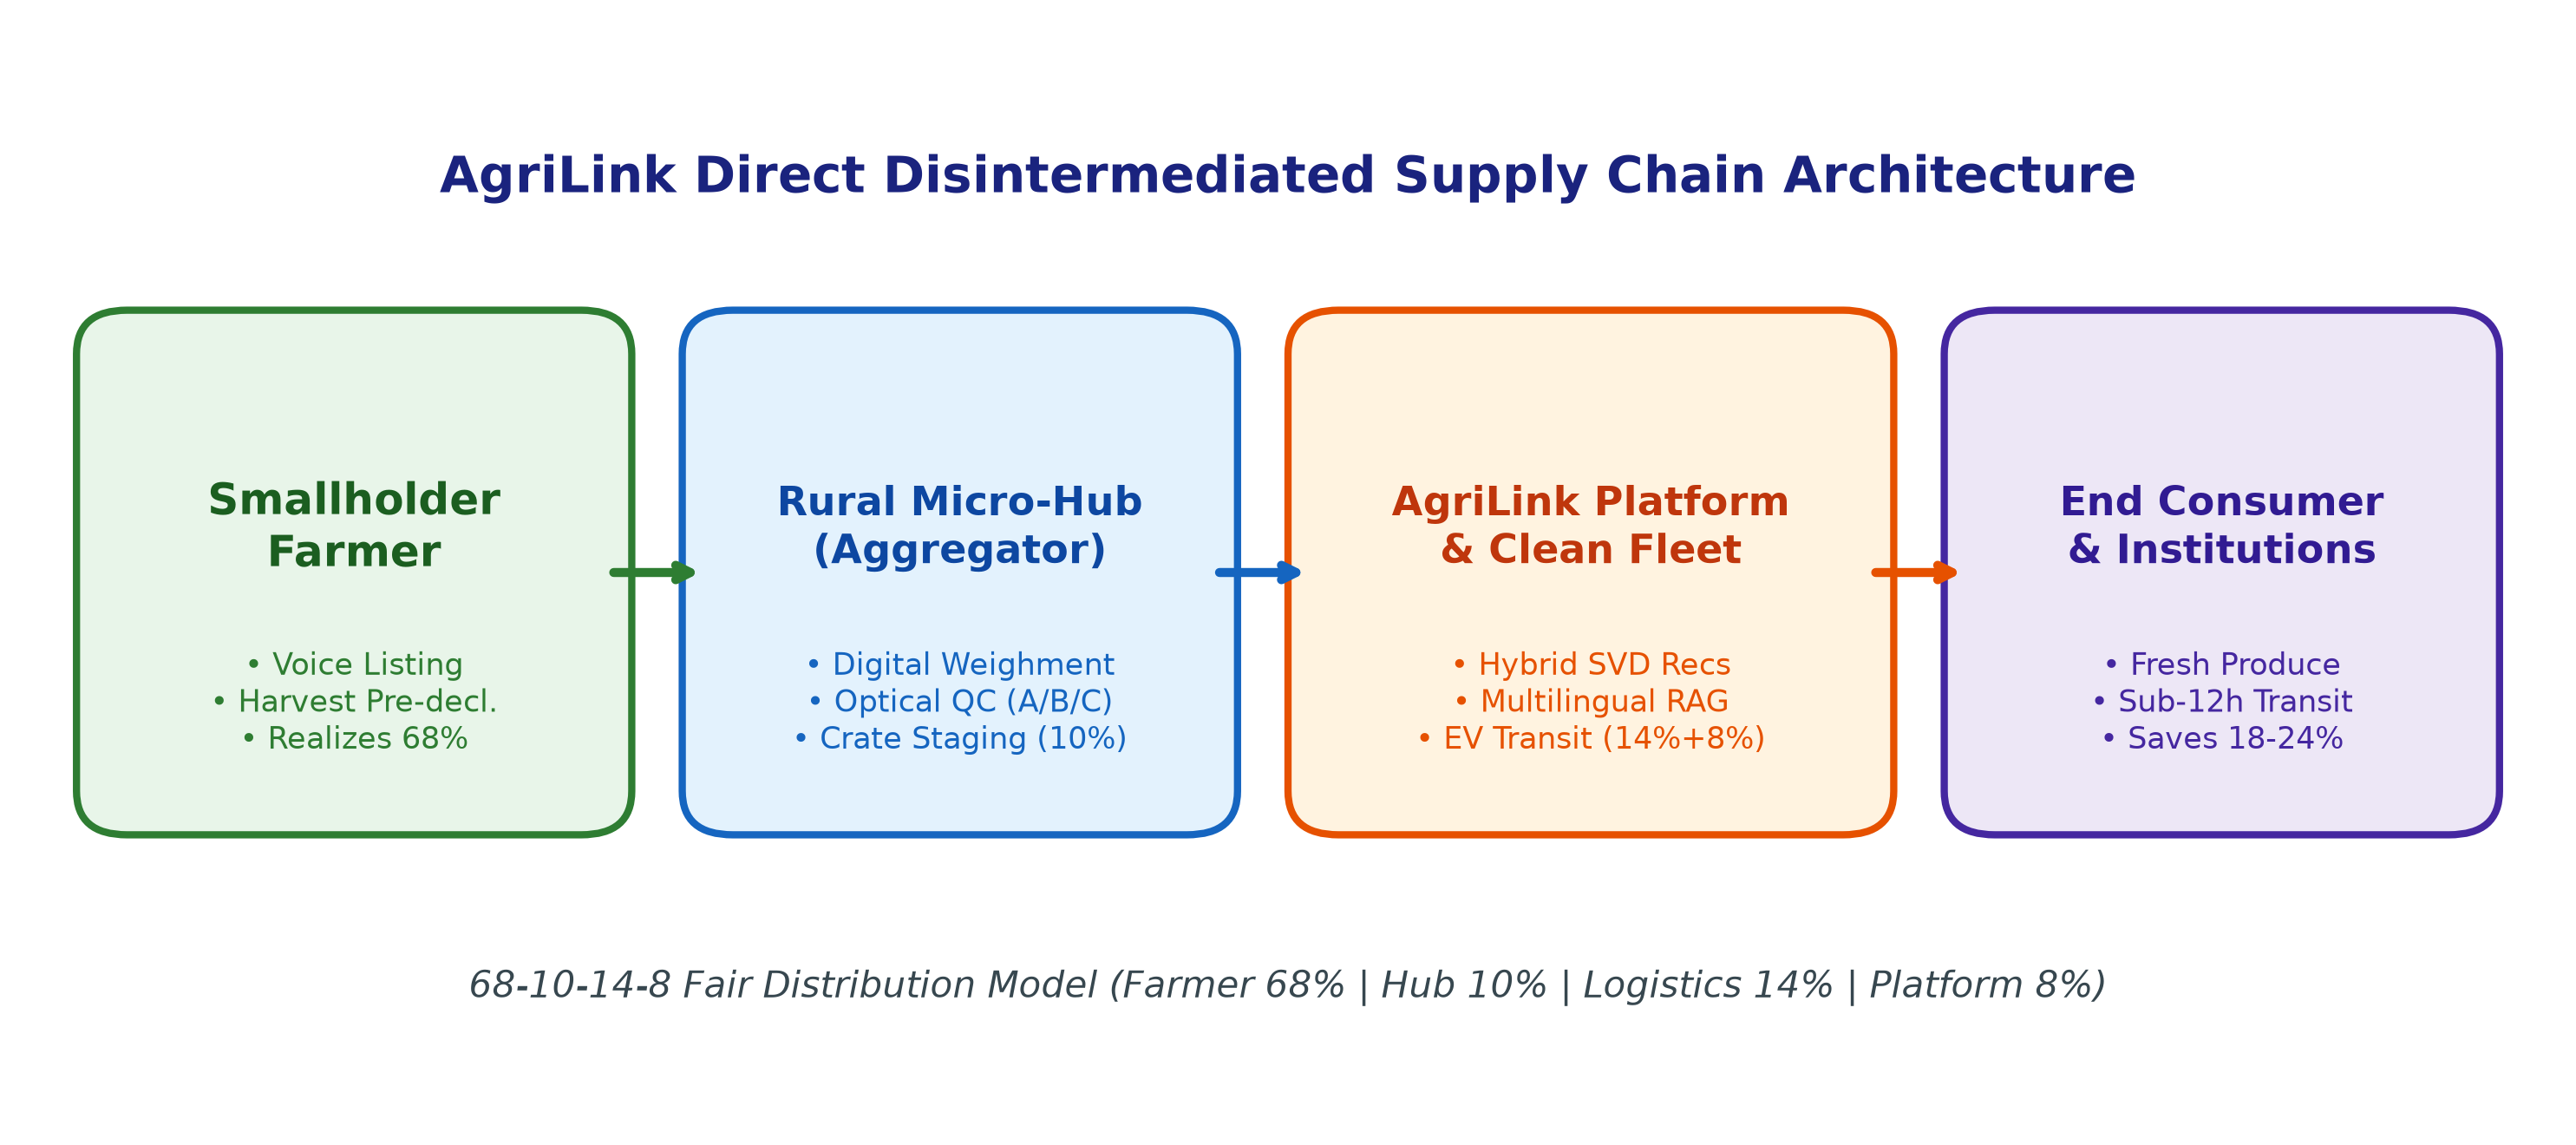
\includegraphics[width=0.75\textwidth]{Figures/C1_Introduction/Figure.png}
	\caption{AgriLink End-to-End Market Disintermediation and Fair-Share Supply Architecture.}
	\label{fig:agrilink_context}
\end{figure}

To formalize this challenge, AgriLink models the supply chain as a multi-tier optimization graph as depicted in Fig. \ref{fig:agrilink_context}. The platform directly connects verified farmers with rural aggregation hubs, route-optimized clean electric fleets, and end consumers under a mathematically regulated 68-10-14-8 revenue distribution model. As analyzed in Section \ref{sec:prob_stmt}, replacing predatory middleman markups with verifiable smart contract logic guarantees that 68\% of every consumer rupee is directly disbursed to the grower's Unified Payments Interface (UPI) account.

\section{Objectives}
\label{sec:Obj}
To achieve comprehensive market disintermediation and automated decision support, the AgriLink platform is architected around four specific technical objectives:

\begin{enumerate}[label=\textbf{Objective \arabic*:}, leftmargin=2.5cm]
	\item \textbf{Direct Multi-Sided Marketplace and Enterprise Relational Backbone}: Design and implement a robust, normalized Third Normal Form (3NF) and Boyce-Codd Normal Form (BCNF) PostgreSQL data platform supporting multi-tenant role-based access for Farmers, Buyers, Rural Aggregators, Logistics Riders, and Administrators with strict Row-Level Security (RLS).
	
	\item \textbf{Dual-Stage Hybrid Recommendation Engine}: Formulate and deploy an intelligent recommendation system uniting Truncated Singular Value Decomposition (SVD) matrix factorization with Term Frequency-Inverse Document Frequency (TF-IDF) content filtering and FP-Growth association rules to solve cold-start challenges for seasonal perishable crops.
	
	\item \textbf{Multilingual Speech-Driven Agricultural Advisory Pipeline}: Construct an end-to-end conversational voice assistant integrating Whisper Automatic Speech Recognition (ASR), AI4Bharat IndicTrans2 translation, and dense FAISS vector indexing to provide low-latency, dialect-aware crop and pest advisory in Kannada, Telugu, Hindi, Malayalam, and English.
	
	\item \textbf{Fair-Share Dynamic Pricing and Capacitated Micro-Hub Logistics}: Formulate an algorithmic fair-price discovery model benchmarking APMC modal indices with empirical quality grading and organic markups, integrated with Capacitated Vehicle Routing Problem (VRP) algorithms to contract transit losses below 10\%.
\end{enumerate}

The functional components embodying these four primary objectives are illustrated in the multi-panel overview shown in Fig. \ref{fig:fig_sub_fig}. Specific aspects of the platform include the direct marketplace interface shown in Fig. \ref{fig:subfig1}, the latent factor recommendation architecture depicted in Fig. \ref{fig:subfig2}, the multilingual speech advisory workflow in Fig. \ref{fig:subfig3}, and the cold-hub routing and ledger infrastructure highlighted in Fig. \ref{fig:subfig4}.

\begin{figure}[t]
\centering
	\begin{subfigure}[t]{0.45\textwidth}
		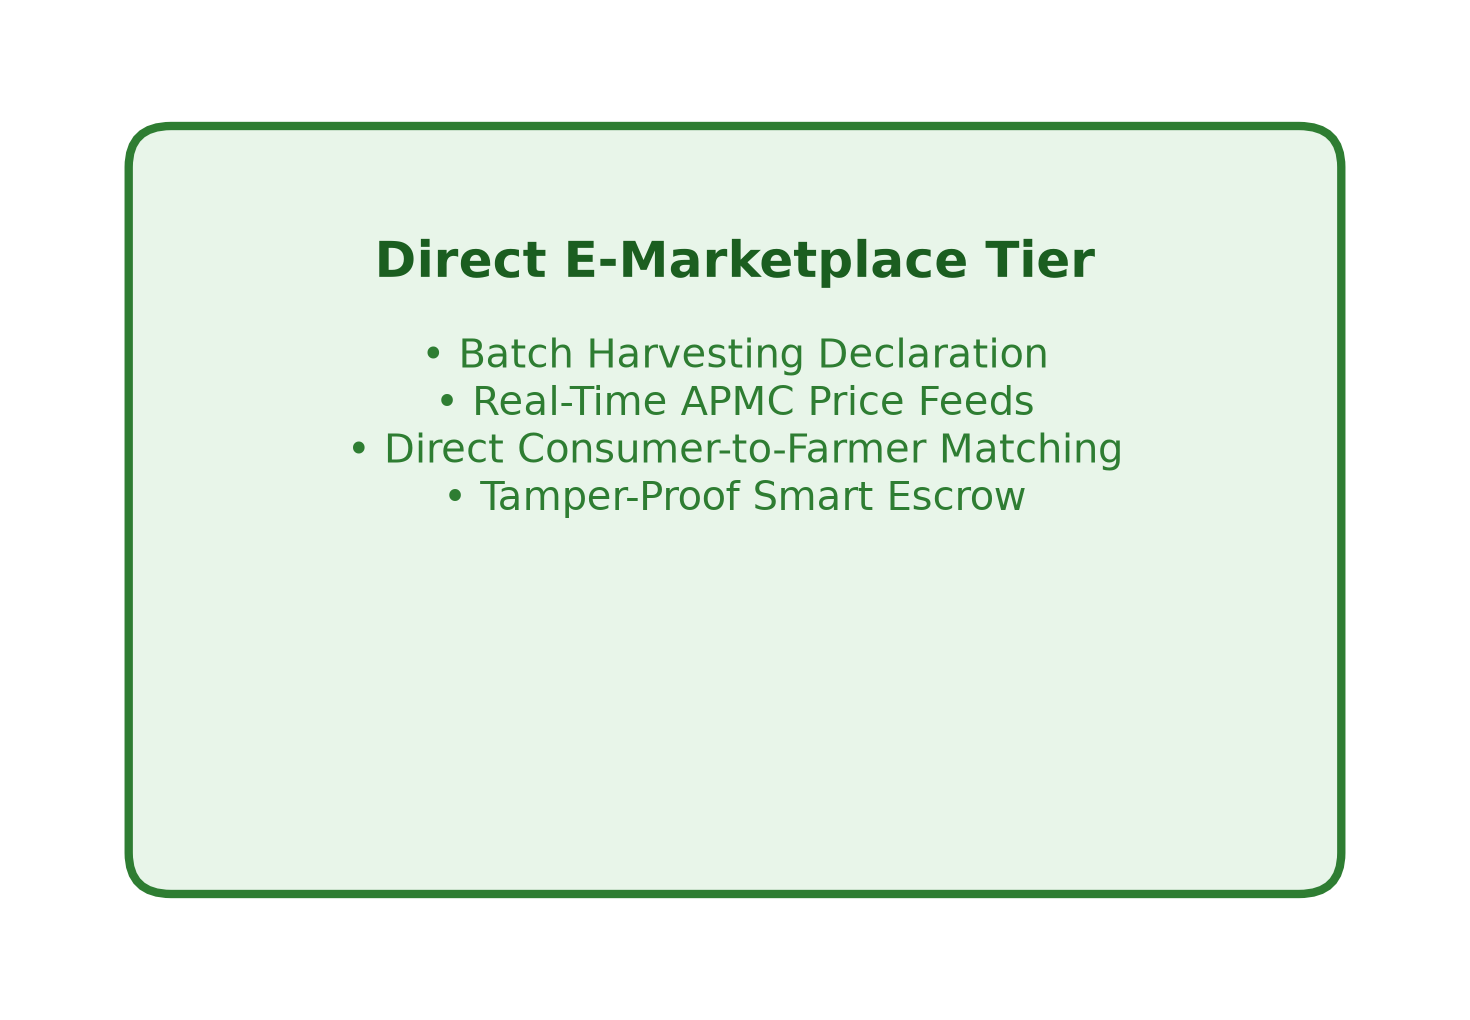
\includegraphics[width=\textwidth]{Figures/C1_Introduction/subfig1.png}
		\caption{Direct Farmgate Marketplace Tier}
		\label{fig:subfig1}
	\end{subfigure}\hspace{0.8cm}
	\begin{subfigure}[t]{0.45\textwidth}
		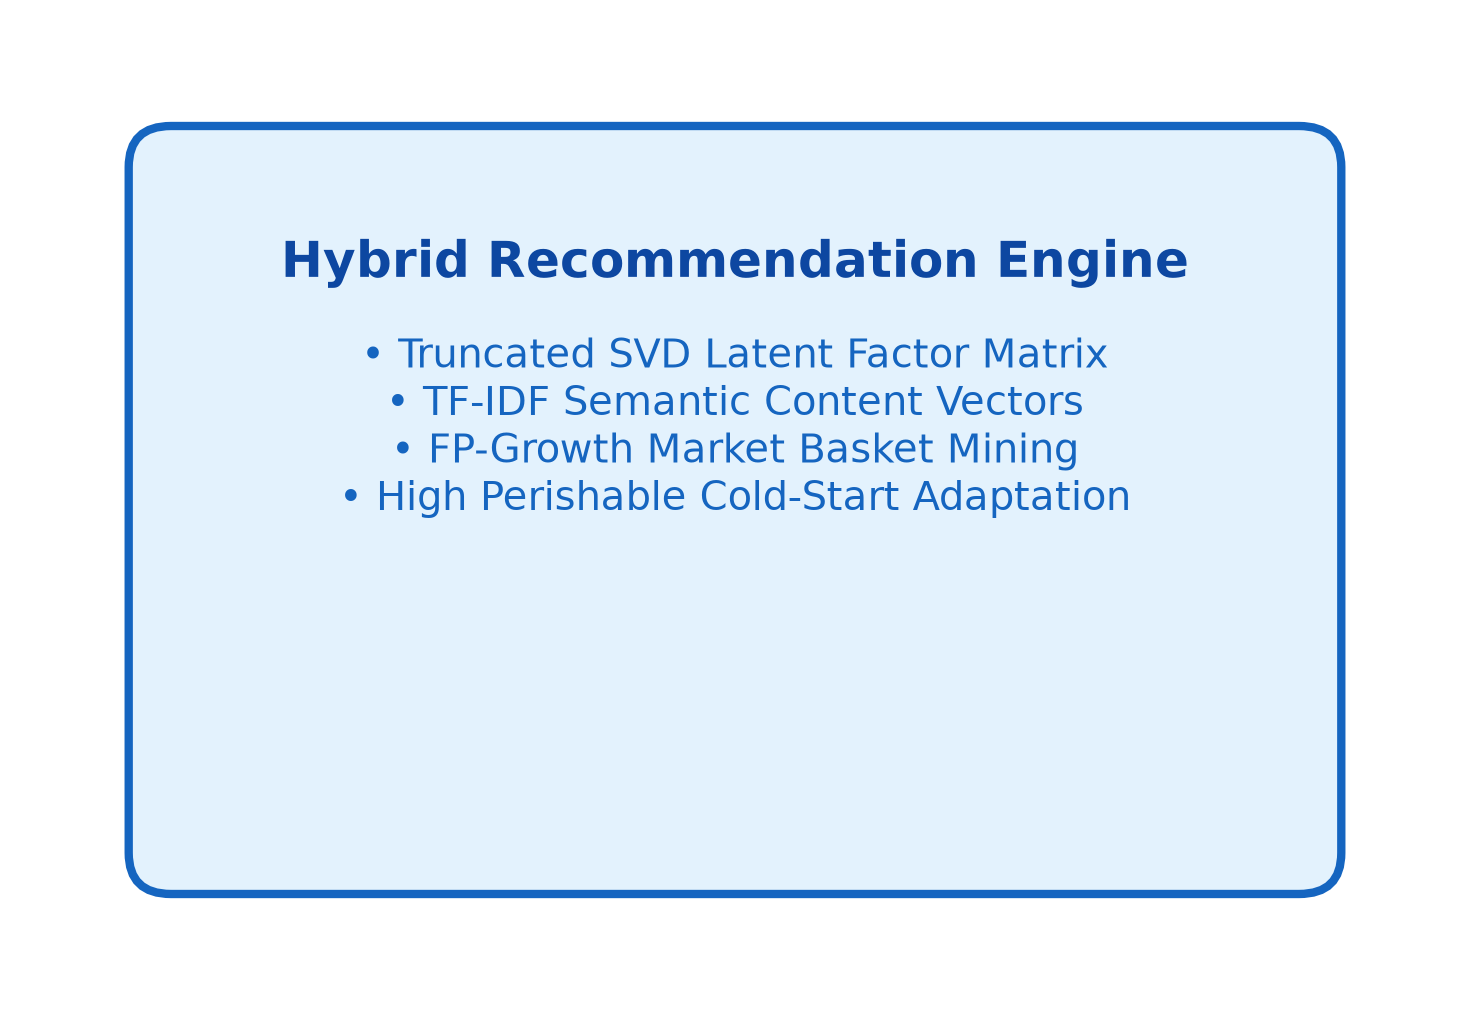
\includegraphics[width=\textwidth]{Figures/C1_Introduction/subfig2.png}
		\caption{Hybrid Recommendation Engine}
		\label{fig:subfig2}
	\end{subfigure}
	
\vspace{0.5cm}

	\begin{subfigure}[t]{0.45\textwidth}
		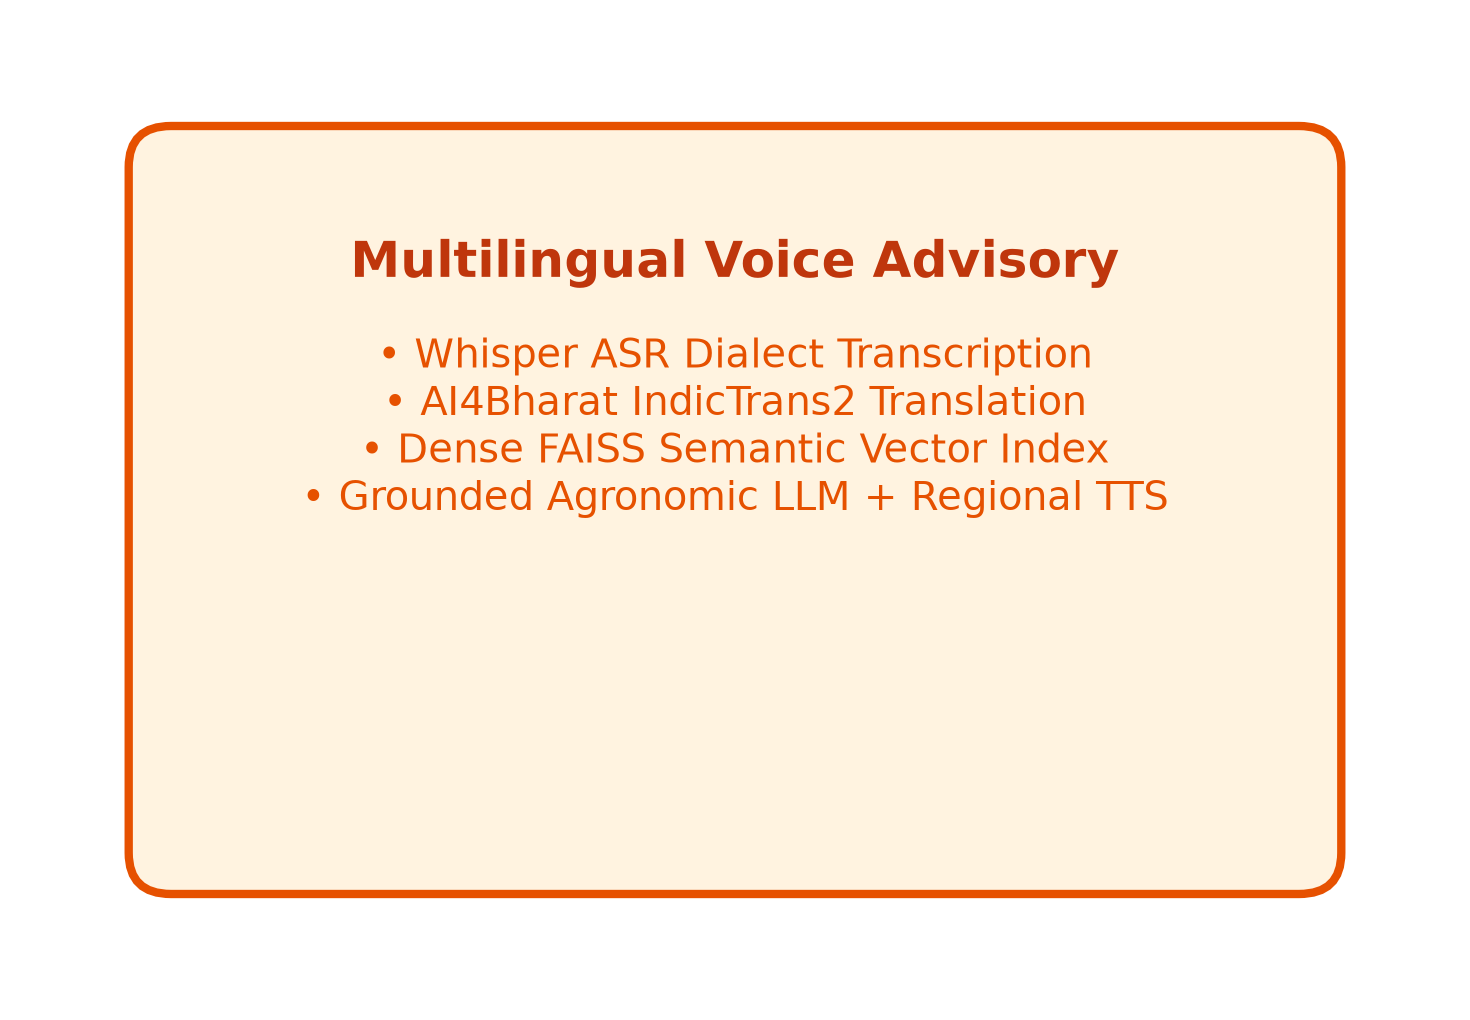
\includegraphics[width=\textwidth]{Figures/C1_Introduction/subfig3.png}
		\caption{Multilingual Voice Advisory Pipeline}
		\label{fig:subfig3}
	\end{subfigure}\hspace{0.8cm}
	\begin{subfigure}[t]{0.45\textwidth}
		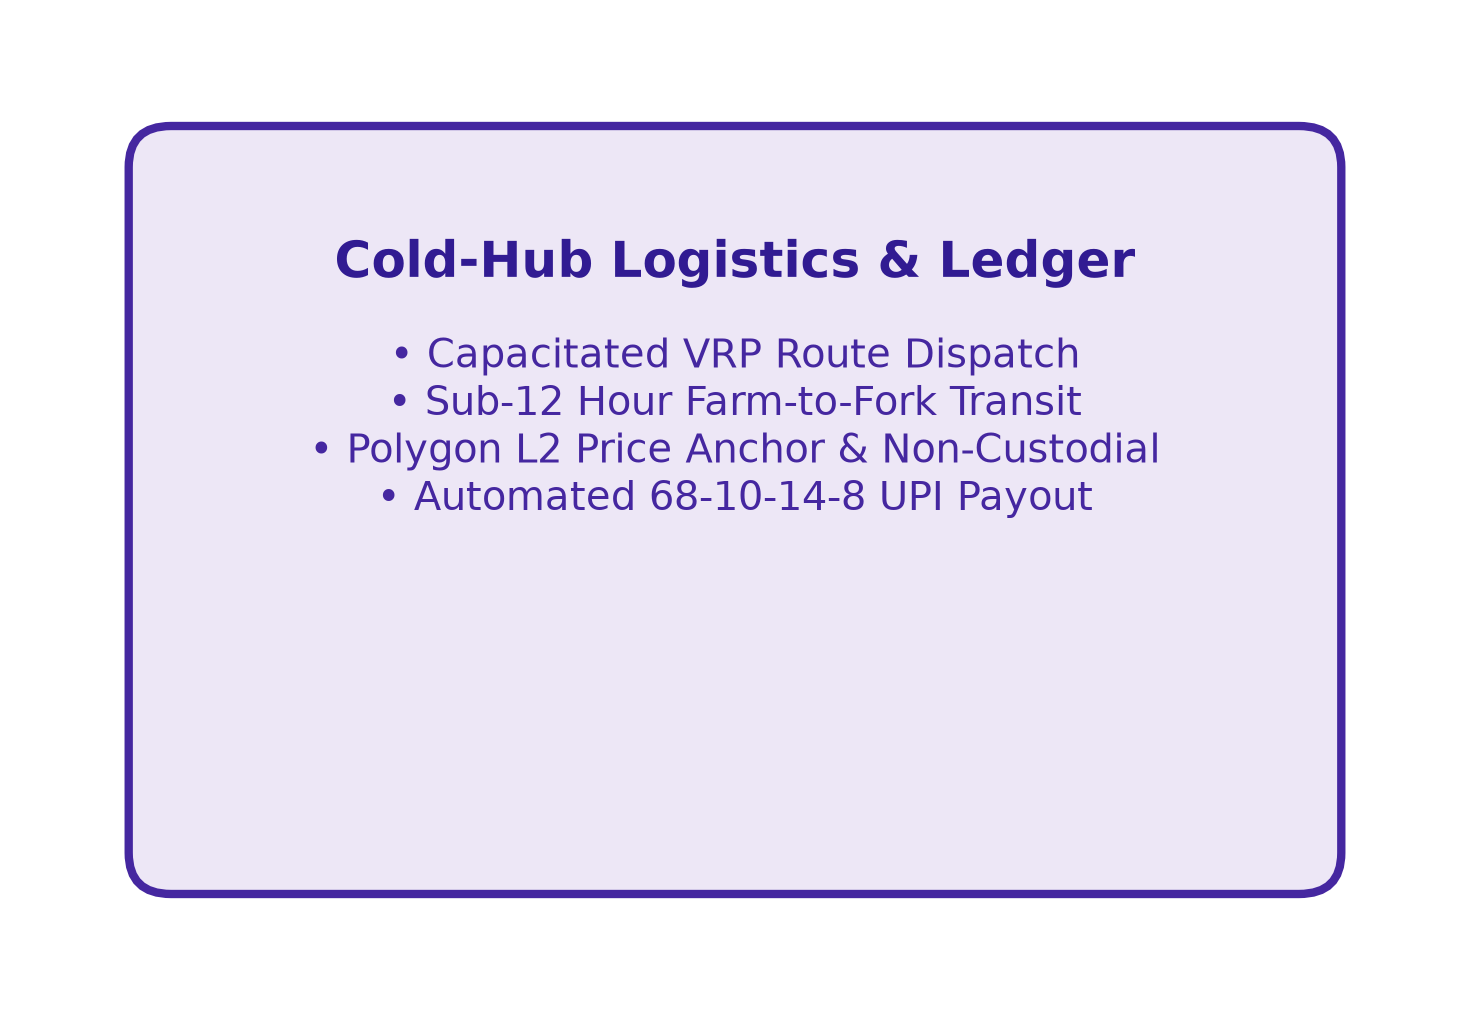
\includegraphics[width=\textwidth]{Figures/C1_Introduction/subfig4.png}
		\caption{Cold-Hub Logistics \& Ledger Tier}
		\label{fig:subfig4}
	\end{subfigure}
	\caption{AgriLink Core Technical Subsystems: (a) Subfigure 1: Direct Farmgate Marketplace Tier; (b) Subfigure 2: Hybrid SVD + Content Recommendation Engine; (c) Subfigure 3: Multilingual Voice Advisory Pipeline; (d) Subfigure 4: Cold-Hub Logistics and Blockchain Ledger Tier.}
	\label{fig:fig_sub_fig}
\end{figure}

This interdisciplinary investigation has been developed and evaluated under the academic oversight of the School of Engineering and Technology at \href{https://vidyashilp.edu.in/}{Vidyashilp University}, Bangalore.

\chapterend